\subsubsection{\stid{1.08} Legion}

\paragraph{Overview}
The Legion project focuses on the development of the Legion runtime system and programming
model. Our focus is on providing the base capabilities of an alternative task-based 
programming model that seeks to improve the amount of available parallelism and enable a 
separation of concerns of the implementation of a task from how that task and its 
associated data are mapped onto a given system architecture.  Our efforts have focused on 
addressing bugs and adding new features to the implementation but also supporting 
applications that are interested in or already using Legion. 

The Legion programming system is freely available via an open source license on the GitLab
site: \url{https://gitlab.com/StanfordLegion/legion}.

\paragraph{Key Challenges}
Legion focuses on providing a programming model and supporting implementation that will 
help address the challenges applications will face in realizing sustained performance on
what are projected to be the nature of Exascale systems. Increased scales combined with 
the challenges of programming potentially diverse accelerator and node-level processor 
technologies are responsible for a significant challenge that has yet to be fully addressed
by today's most prominent programming systems -- none of which have been fully validated 
on \emph{yet-to-be-determined} system architectures for the Exascale era of computing. 

\paragraph{Solution Strategy}
In funded collaboration between Los Alamos and Stanford University we are providing not
only the implementation of the Legion programming model but also numerous opportunities 
for application developers and participants in the ECP PathForward efforts to learn about 
Legion and data-flow and task-based approaches to programming.  We also closely work with
Combustion-Pele (AD 2.2.2.02) and the data analytics efforts in support of ExaFEL (AD 2.2.4.05)
to provide bug fixes, performance optimizations and implementation help.  We work with 
these applications and are exploring Legion with a few others, and in collaboration with 
the LANL ATDM Programming Models and Runtimes project (ST 2.3.1.02), to identify needs 
and missing features in the programming model and runtime implementation.  In addition, 
we also look at numerous aspects of having the Legion system interoperate with today's 
more widely used programming systems -- e.g. MPI and OpenMP.  This is critical in terms of
providing a path for adoption and experimentation to occur in a more productive fashion.
Finally, we are also actively exploring techniques for simplifying Legion programming to 
help assist in not only potential adoption but also in helping to educate the broader 
community about the programming model and its advantages on Exascale-class systems. 

\paragraph{Recent Progress}

Our most recent progress has been devoted to getting the S3D DNS combustion application 
running on the Summit system at OLCF and the Piz Daint system at the Swiss National 
Supercomputing Centre.  This work is utilizing the most recent version of Legion with a 
goal of both bug, scaling and overall performance enhancements.  This effort is an update
that covers new science relative to our previous work that has recently been 
published~\cite{Treichler:2017}.  At present the full set of performance and application
characteristics for this effort are still being analyzed and in particular, issues
encountered on Summit are being discussed with OLCF staff.  A early look at rough 
numbers suggest anywhere from a $26$ to over $100$X boost in performance over the 
\emph{production} (MPI-based) version of S3D.  Additional Legion features worked on in 
collaboration with LANL's ATDM efforts (ST 2.3.1.02) have resulted in much improved 
scaling capabilities due to reduced runtime overheads in comparison to past work.

Figure~\ref{fig:task-graph} on the following page, shows the task graph for a single time 
step on one node of the Legion implementation of S3D simulating an n-dodecane reaction.  
We hope to soon be able to release a more detailed analysis of the new Legion-S3D runs. 

\begin{figure}[htb]
	\centering
	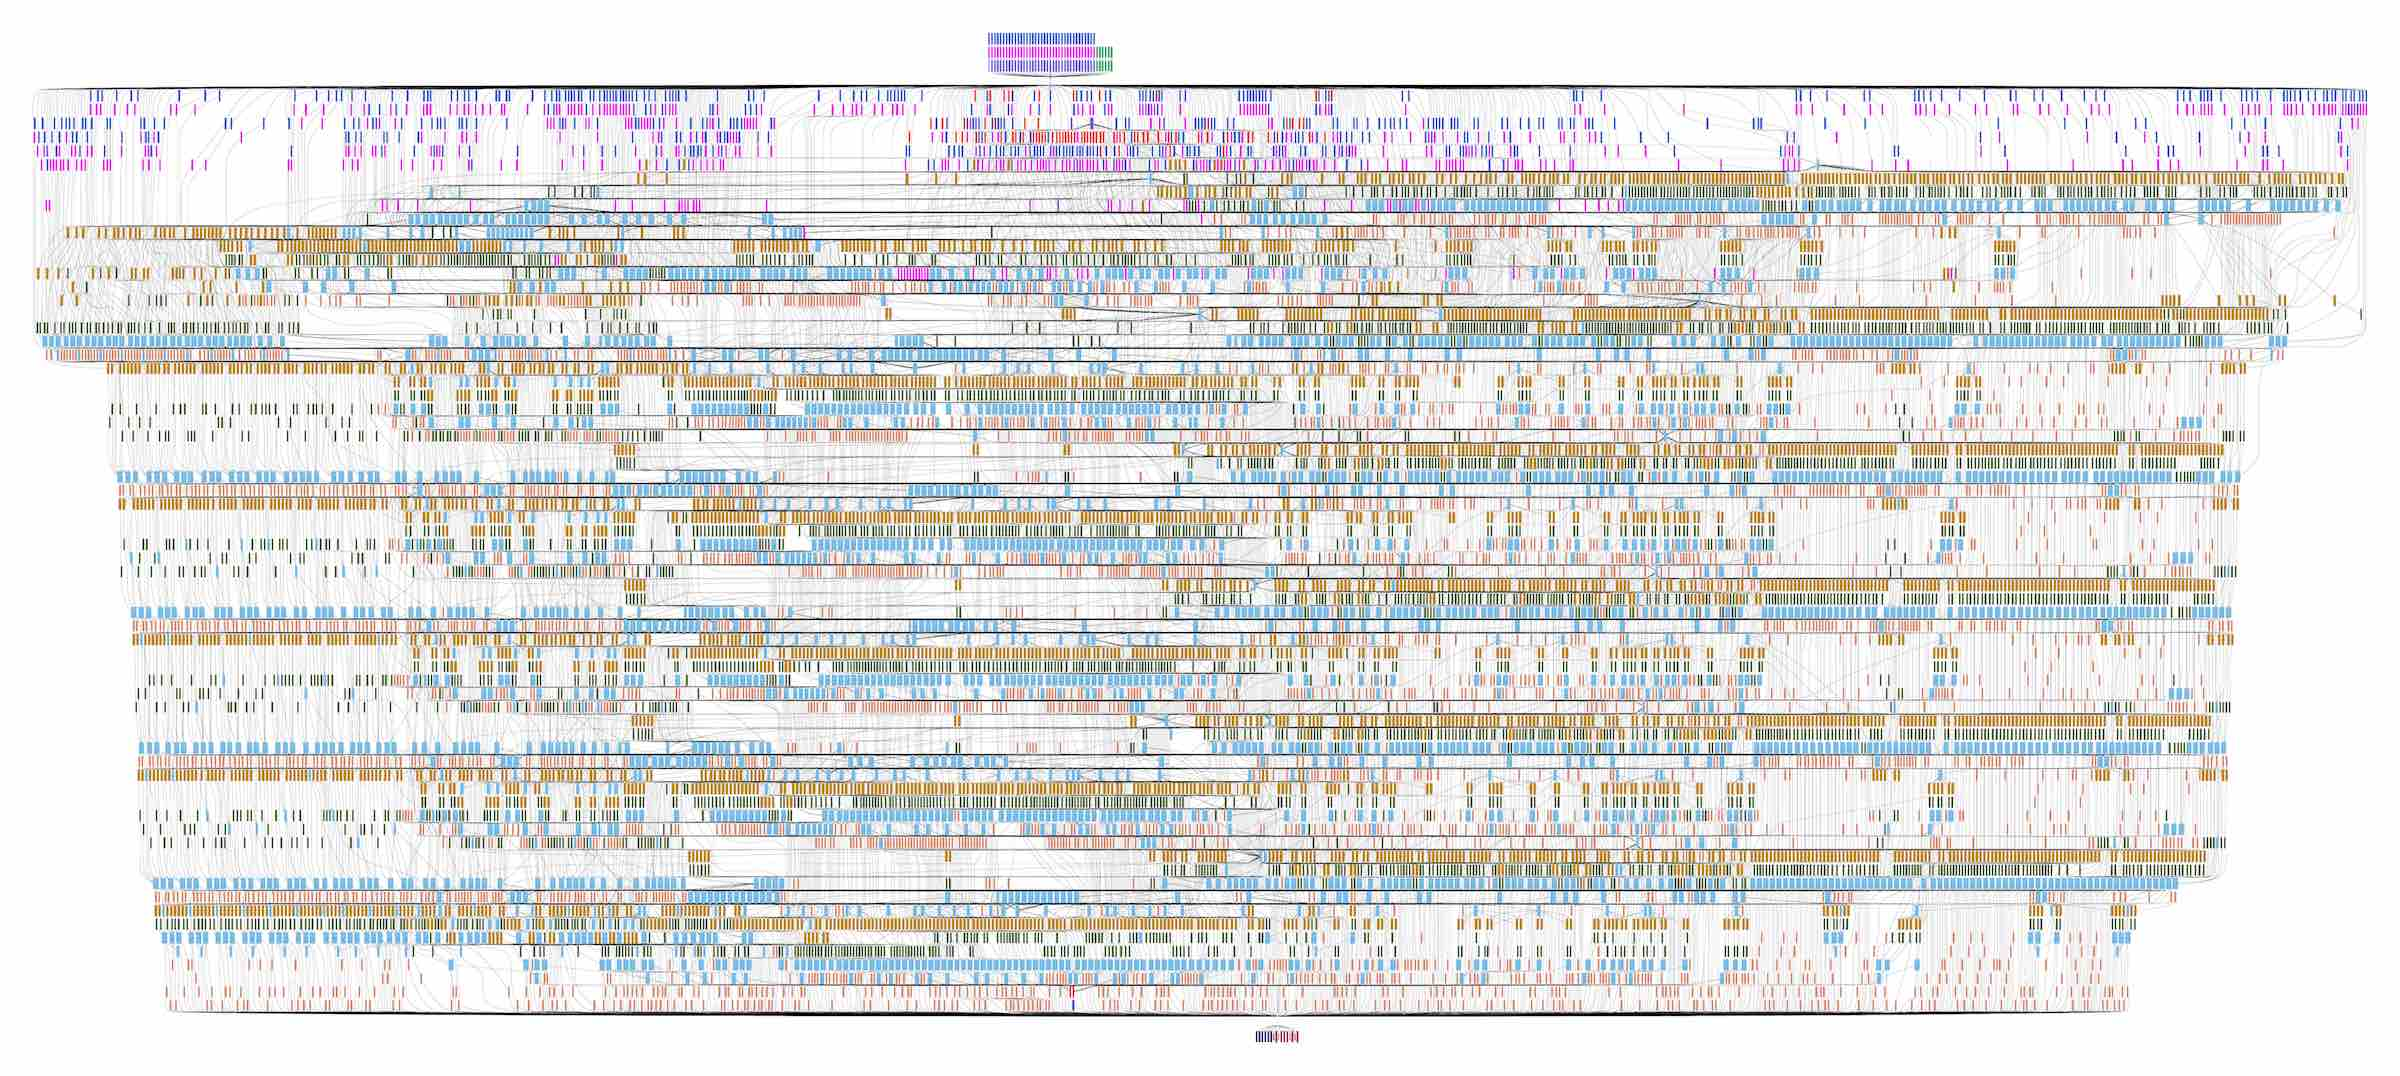
\includegraphics[width=6.5in]{projects/2.3.1-PMR/2.3.1.08-Legion/tg}
	\caption{\label{fig:task-graph}The Legion task graph for a single time step on a 
	single node.  The S3D configuration in this example is simulating n-dodecane 
	chemistry reactions in addition to the direct numerical simulation of the 
	turbulent flow.}
\end{figure}

\paragraph{Next Steps}
We will continue to focus on improving the interoperability of Legion with other programming
systems, simplifying the programming API for the Legion runtime to improve both our educational 
outreach as well as developer productivity, have regular open source releases of Legion and
also work with application teams for debugging, feature improvements and performance 
tuning.  In addition we are actively monitoring the emerging hardware technology components
that are potential targets for use in the Exascale systems that will be eventually deployed 
by both the DOE Office of Science and the NNSA. 
